\section{Convex Optimization Problems}

Optimal value $f^\star =
	\operatorname{inf}\{f(x)\mid
	g_i(x)\le0,h_j=0 \}$
$f^\star=+\infty$ OP is infeasible,
$f^\star=-\infty$ OP is unbound below

\subsection{Feasibility  Problem}

Special case $f(x)=0,\forall x$
$\Leftrightarrow$
$\min_s$ s.t. $g_i(x)\le s,h_j(x)=0$

\textbf{Linear Programming}
$ \operatorname{minimize} c\T x
	\text{ s.t. } Ax-b \ge 0,\ x\ge0$

Step 1:
$\mathcal{L}(x,\lambda_1,\lambda_2) =
	c\T x-\lambda_1\T (Ax-b) -\lambda_2\T x,\ \lambda_i \ge0$

Step 2:
$\underset{x \in \mathcal{\mathbb{R}}^n}{\operatorname{inf}}
	\mathcal{L}=\lambda_1\T b$
, if $c-A\T\lambda_1-\lambda_2=0$, else $-\infty$

Step 3: Dual,
maximize $b\T\lambda$
s.t.
$c-A\T\lambda\ge0,\lambda\ge0$
(again LP)

\begin{proposition}
	The optimal solution of a linear program (if it exists)
	lies always on the boundary of the feasible set
	and there exists an optimal solution that is a vertex of the feasible set.
\end{proposition}


\textbf{Quadratic Programming}
convex if $P=P\T$ positiv semi-definite
minimize $\frac{1}{2}x\T Px+q\T x$
s.t. $Gx\le h,\ Ax=b$


\textbf{Second-Order Cone Program}

minimize $f\T x \text{ s.t. }
	|A_ix+b|\le c_i\T x+d_i, Fx=g$

Second-order cone
$C_{n+1}=\{ (x,t)\mid
	x\in\mathbb{R}^{n}, t\in \mathbb{R}, |x|\le t \}$

$|A_ix+b|\le c_i\T x+d_i$
$\Leftrightarrow$
$(A_ix+b, c_i\T x+d_i)\in C_{n+1}$

\textbf{Semi-Definite Programming} with symmetric $F_i,X,A_i$

minimize $c\T x$
s.t.
$\sum_{i=1}^{n}x_iF_i+G\preceq0$,
$Ax=b$

\textbf{Standard form}
minimize $\operatorname{tr}(CX)$
s.t.
$X\ge0$,
$\operatorname{tr}(A_iX)=b_i$
$\operatorname{tr}(CX)=\sum_{i=1}^{n}\sum_{j=1}^{n}$
$C_{ij}X_{ij}$,
$C\in\mathbb{R}^{n\times n}$,
$i=1,..,m$

LP$\subset$ QP $\subset$ QCQP
\scriptsize
(Quadratically Constrained QP)
\footnotesize
$\subset$ SOCP $\subset$ SDP

% 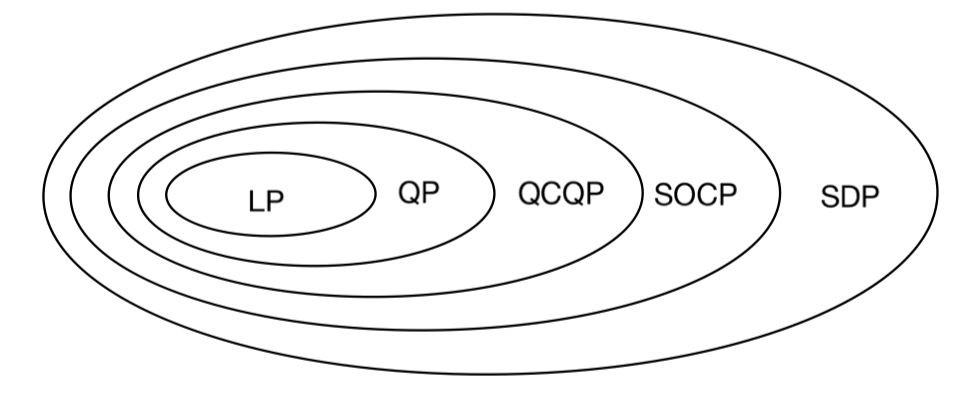
\includegraphics[width=\columnwidth]{images/problem_class.png}








